\chapter{Process Chapter from sw601f15}\label{app:601}\pdfmapline{-dummy LMRoman12-Regular}
\noindent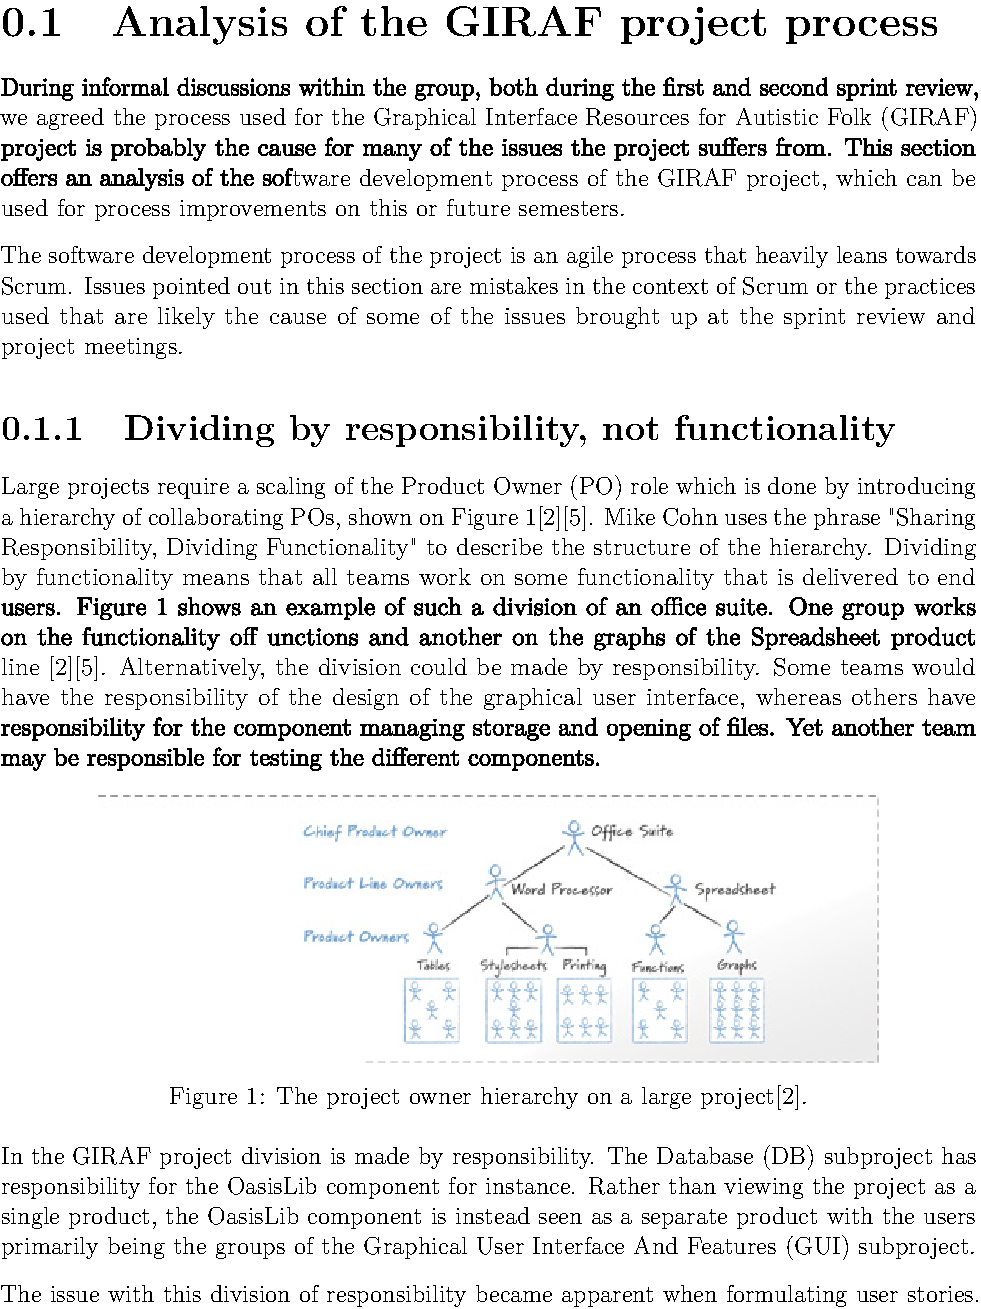
\includegraphics[page=1,width=0.99\textwidth]{part_appendix/sw601f15.pdf}

\noindent\includegraphics[page=2,width=1\textwidth]{part_appendix/sw601f15.pdf}

\noindent\includegraphics[page=3,width=1\textwidth]{part_appendix/sw601f15.pdf}

\noindent\includegraphics[page=4,width=1\textwidth]{part_appendix/sw601f15.pdf}

\noindent\includegraphics[page=5,width=1\textwidth]{part_appendix/sw601f15.pdf}

\noindent\includegraphics[page=6,width=1\textwidth]{part_appendix/sw601f15.pdf}\clearpage{}

\noindent\textsf{NOTE:} This bibliography is part of \appendixref{app:601}. The bibliography of this report can be seen \onpage{bibliography}.
\vspace{1cm}

\noindent\begin{tikzpicture}
    \node[anchor=south west,inner sep=0] (image) at (0,0) {\includegraphics[page=7,width=0.99\textwidth]{part_appendix/sw601f15.pdf}};
    \begin{scope}[x={(image.south east)},y={(image.north west)}]
        \node[rotate=25, fill=yellow, fill opacity=0.20, align=center, text opacity=0.55] (watermark) at (0.5,0.33) {\LARGE\sffamily This bibliography is part of Appendix L};
        \node[rotate=25, fill=yellow, fill opacity=0.20, align=center, text opacity=0.55] (watermark) at (0.5,0.66) {\LARGE\sffamily This bibliography is part of Appendix L};
    \end{scope}
\end{tikzpicture}
%\includegraphics[page=7,width=1\textwidth]{part_appendix/sw601f15.pdf}